% !TEX TS-program = pdflatex
% !TEX encoding = UTF-8 Unicode

% Matthew Urffer Master Thesis
% INTRODUCTORY MATERIAL 

\section{Introduction}

\subsection{Radiation Portal Monitors}

%%%%%%%%%%%%%%%%%%%%%%%%%%%%%%%%%%%%%%%%%%%%%%%%%%%%%%%%%%%%%%%%%%%%%%%%%%%%%%%
\begin{frame}{U.S. Border Traffic}
\begin{columns}[onlytextwidth]
\begin{column} {0.45\textwidth}
 
  \begin{itemize}
  \item Every day 932,456 people cross into the U.S. \cite{cpb_typical_2012}
    \begin{itemize}
    	\item 259,191 by air
	\item 48,073 by sea
	\item 621,874 by land
    \end{itemize}
  \item 64,483 truck, rail and sea containers \cite{cpb_typical_2012}
 \item 253,821 privately-owned vehicles \cite{cpb_typical_2012}
  \end{itemize}
\end{column}
\begin{column}{0.45\textwidth}
\centering
\begin{figure}
		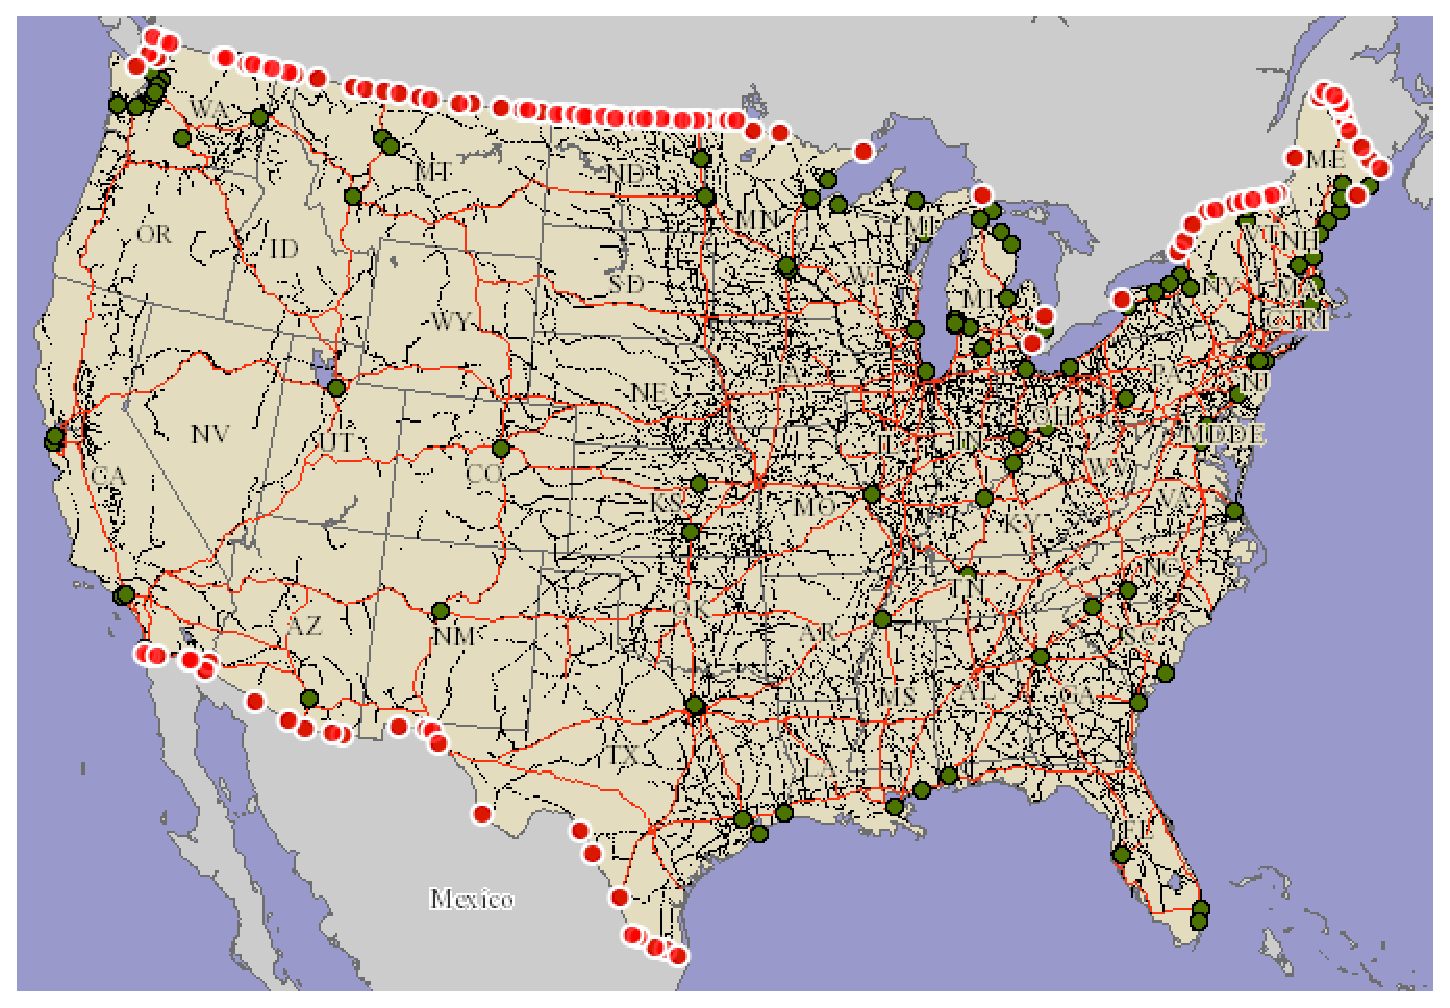
\includegraphics[width=\textwidth]{images/PortalEntryMap.eps}
		\label{fig:PortalEntryMap}
	\caption{Portal Entry Points into the U.S.}
\end{figure}
\end{column}
\end{columns}
\end{frame}

%%%%%%%%%%%%%%%%%%%%%%%%%%%%%%%%%%%%%%%%%%%%%%%%%%%%%%%%%%%%%%%%%%%%%%%%%%%%%%%
\begin{frame}{Radiation Portal Monitors}
\begin{columns}[onlytextwidth]
	\begin{column} {0.45\textwidth}
  	\begin{itemize}
  		\item Radiation portal monitors (RPMs) are passive radiation detectors
  		\item {
  			 RPMs are currently   ${}^3$He based detectors
  			\center
    		${}^3He +n \to p +{}^3H$
    	}
  		\item 
  			Shortage of ${}^3$He, so alternatives are being explored
  		\end{itemize}
	\end{column}
	\begin{column}{0.5\textwidth}
		\centering
		\begin{figure}
			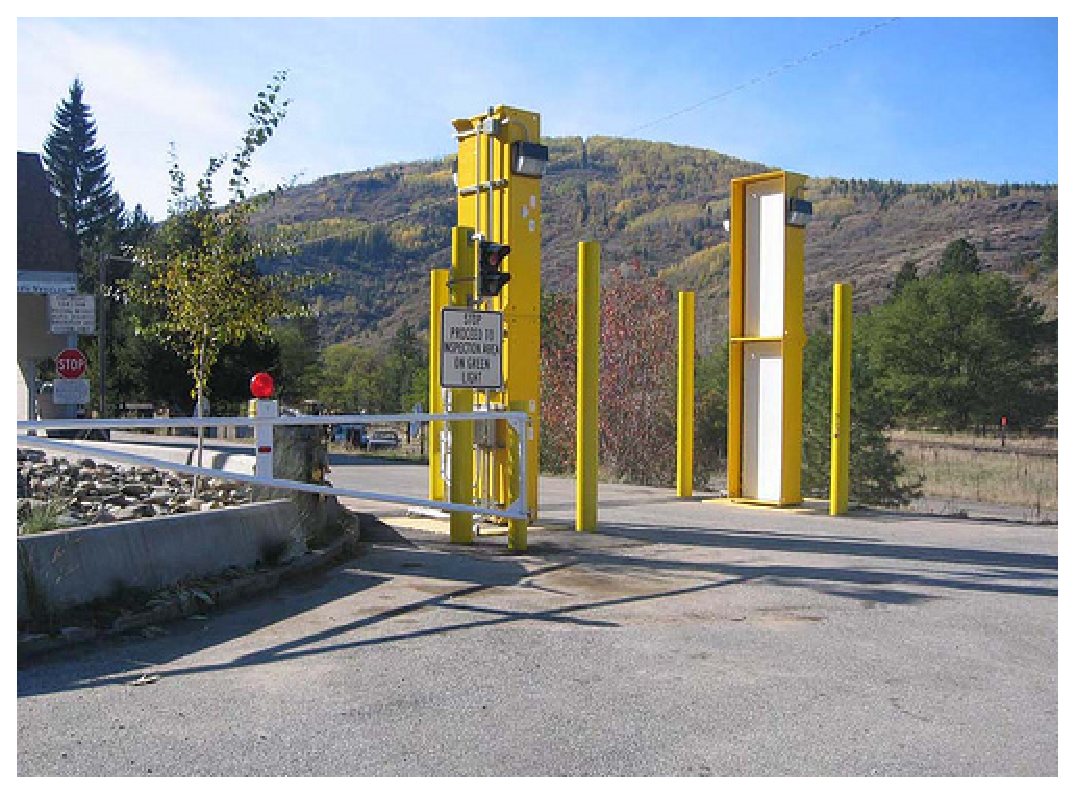
\includegraphics[width=\textwidth]{images/RPM8_Installed.eps}
			\label{fig:RPM8Installed}
			\caption{Installed RPM}
			\end{figure}
	\end{column}
\end{columns}
\end{frame}


%%%%%%%%%%%%%%%%%%%%%%%%%%%%%%%%%%%%%%%%%%%%%%%%%%%%%%%%%%%%%%%%%%%%%%%%%%%%%%%
\begin{frame}{Neutron Adsorption Interactions}
\begin{itemize}
	\item Desired reaction properties
	\begin{itemize}
		\item High probability of occurrence
		\item Ease of detecting reaction products
		\item Reaction products have a low pulse height defect
	\end{itemize}
\end{itemize}
\begin{table}
	\tiny
	\begin{tabular}{ c | c c c} 
		Reaction                           & Q-Value (MeV) & Thermal Cross Section & Application \\
		\hline
		\hline
		${}^3He + n \to p +{}^3H$          & 0.756     & 5,330 & Proportional counter gas \\
		${}^6Li + n \to {}^3H + \alpha$    & 4.78      & 940 & Lithium glass scintillators \\
		${}^{10}B + n \to \alpha + {}^7Li$ & 2.31      & 3,840 & Plastic scintillators \\
		${}^{157}Gd + n \to \gamma$        &various    & 259,000 & various \\
	\end{tabular}
\end{table}
\end{frame}

%%%%%%%%%%%%%%%%%%%%%%%%%%%%%%%%%%%%%%%%%%%%%%%%%%%%%%%%%%%%%%%%%%%%%%%%%%%%%%%
\begin{frame}{Energy Deposition (Charged Particle)}
Products of ${}^6$Li neutron interaction are triton and alpha:
\begin{columns}[onlytextwidth]
\begin{column}{0.45\textwidth}
\begin{itemize}
	\small
	\item Alpha Energy: 2.05 MeV
	\item Triton Energy: 2.73 MeV
\end{itemize}
Alpha and tritons tend to deposit all of their energy in a small region
\end{column}
\begin{column}{0.45\textwidth}
	\begin{figure}
	\includegraphics[width=\textwidth]{images/PStarAStarRange.eps}
	\caption{Alpha and Triton Range (CSDA) \protect \cite{berger_estar_2005}}
	\label{fig:PStarAStarRange}
	\end{figure}
\end{column}
\end{columns}
\end{frame}

\subsection{Detector Requirements}
%%%%%%%%%%%%%%%%%%%%%%%%%%%%%%%%%%%%%%%%%%%%%%%%%%%%%%%%%%%%%%%%%%%%%%%%%%%%%%%
\begin{frame}{Detector Requirements}
DHS / DNDO (along with PNNL) has determined a set of objectives that replacement technologies should meet:
\begin{table}
	\tiny
	\begin{tabular}{c c }
	Parameter & Specification \\
	\hline
	\hline
	Absolute neutron detection efficiency & 2.5 cps/ng of ${}^{252}Cf$ (in specified test configuration) \\
	Intrinsic gamma-neutron detection efficiency & $ \epsilon_{int,\gamma}\leq 10^{-6}$ \\
	Gamma absolute rejection ratio for neutrons (GARRn) & $ 0.9 \leq \text{ GARRn }\leq$ 1.1 at 10 mR/h exposure \\
	Cost &  \$ 30,000 per system \\
	\hline
	\end{tabular}
\end{table}
\end{frame}

%%%%%%%%%%%%%%%%%%%%%%%%%%%%%%%%%%%%%%%%%%%%%%%%%%%%%%%%%%%%%%%%%%%%%%%%%%%%%%%
\begin{frame}{Absolute Neutron Efficiency}
\newtheorem{thm1}{Absolute Neutron Efficiency}
\begin{thm1}<1->
$$\epsilon_{abs} = \frac{\text{Counts}}{\text{Quanta Radiation Emitted}}\; \; \protect \cite{knoll_radiation_2009} $$
Constraint:
$$\epsilon_{abs} \geq 2.5\; \text{cps per ng}\; {}^{252}\text{Cf}$$
\end{thm1}
Test configuration is defined to be 1 ng ${}^{252}$Cf surrounded by 0.5 cm of lead and 2.5 cm of HDPE, with the detector midpoint 2 m from the source \cite{kouzes_alternative_2010}
\end{frame}


%%%%%%%%%%%%%%%%%%%%%%%%%%%%%%%%%%%%%%%%%%%%%%%%%%%%%%%%%%%%%%%%%%%%%%%%%%%%%%%
\begin{frame}{Intrinsic Gamma-Neutron Detection Efficiency}
\newtheorem{thm2}{Intrinsic Gamma-Neutron Detection Efficiency}
\begin{thm2}<1->
$$\epsilon_{int,n \gamma} = \frac{\text{Counts}}{\text{Quanta Radiation Crossing Detector}} \; \protect \cite{kouzes_alternative_2010} $$
Constraint:
$$ \epsilon_{int,n \gamma} \leq 10^{-6} $$
\end{thm2}
\begin{itemize}
	\item Counts over quanta crossing the detector
	\item Measured from a source that produces a 10 mR/hr field
\end{itemize}
\end{frame}

%%%%%%%%%%%%%%%%%%%%%%%%%%%%%%%%%%%%%%%%%%%%%%%%%%%%%%%%%%%%%%%%%%%%%%%%%%%%%%%
\begin{frame}{Gamma Absolute Rejection Ratio}
\newtheorem{thm3}{GARRn}
\begin{thm3}<1->
$$ GARRn = \frac{\epsilon_{\gamma,abs}}{\epsilon_{n,abs}} \; \protect \cite{kouzes_alternative_2010} $$
Constraint:
$$ 0.9 \leq GARRn \leq 1.1 $$
\end{thm3}
The detector's performance should change by no more than 10\% in a strong gamma field
\begin{itemize}
	\item GARRn is measured by exposing the detector to a 10 mR/hr gamma field while exposed to neutron source
	\item Count rate is measured when the gamma source is no longer present
	\item Difference determines the GARRn
\end{itemize}
\end{frame}

%%%%%%%%%%%%%%%%%%%%%%%%%%%%%%%%%%%%%%%%%%%%%%%%%%%%%%%%%%%%%%%%%%%%%%%%%%%%%%%
%                                                                             %
%                                PREVIOUS WORK                                %
%                                                                             %
%%%%%%%%%%%%%%%%%%%%%%%%%%%%%%%%%%%%%%%%%%%%%%%%%%%%%%%%%%%%%%%%%%%%%%%%%%%%%%%
\subsection{Previous Work}

%%%%%%%%%%%%%%%%%%%%%%%%%%%%%%%%%%%%%%%%%%%%%%%%%%%%%%%%%%%%%%%%%%%%%%%%%%%%%%%
\begin{frame}{Replacement Technologies (Boron)}
\begin{columns}[onlytextwidth]
\begin{column}{0.45\textwidth}
\begin{itemize}
	\small
	\item Boron Straw Tubes (Proportional Technology) \cite{kouzes_boron-lined_2012}
	\begin{itemize}
		\tiny
		\item Count rate meets requirements
		\item Gamma rejection is estimated to be $4x10^{-9}$
		\item GARRn within desired range
	\end{itemize}
	\small
	\item Boron Triflouride Gas Detectors (LND) \cite{kouzes_bf3_2009}
	\begin{itemize}
		\tiny
        \item Two tubes are marginally able to replace one ${}^3$He tube
		\item BF${}_3$ Tubes require 2200V to operate than ${}^3$He tubes (1000 V)
		\item BF${}_3$ Tubes require less pressure than ${}^3$He tubes
	\end{itemize}
\end{itemize}
\end{column}
\begin{column}{0.45\textwidth}
	\begin{figure}
	\centering
		\includegraphics[height=0.25\textheight]{images/B10StrawFibers.eps}
		\caption{ ${}^{10}$B Straw Fibers}
		\label{fig:B10StrawFibers}
		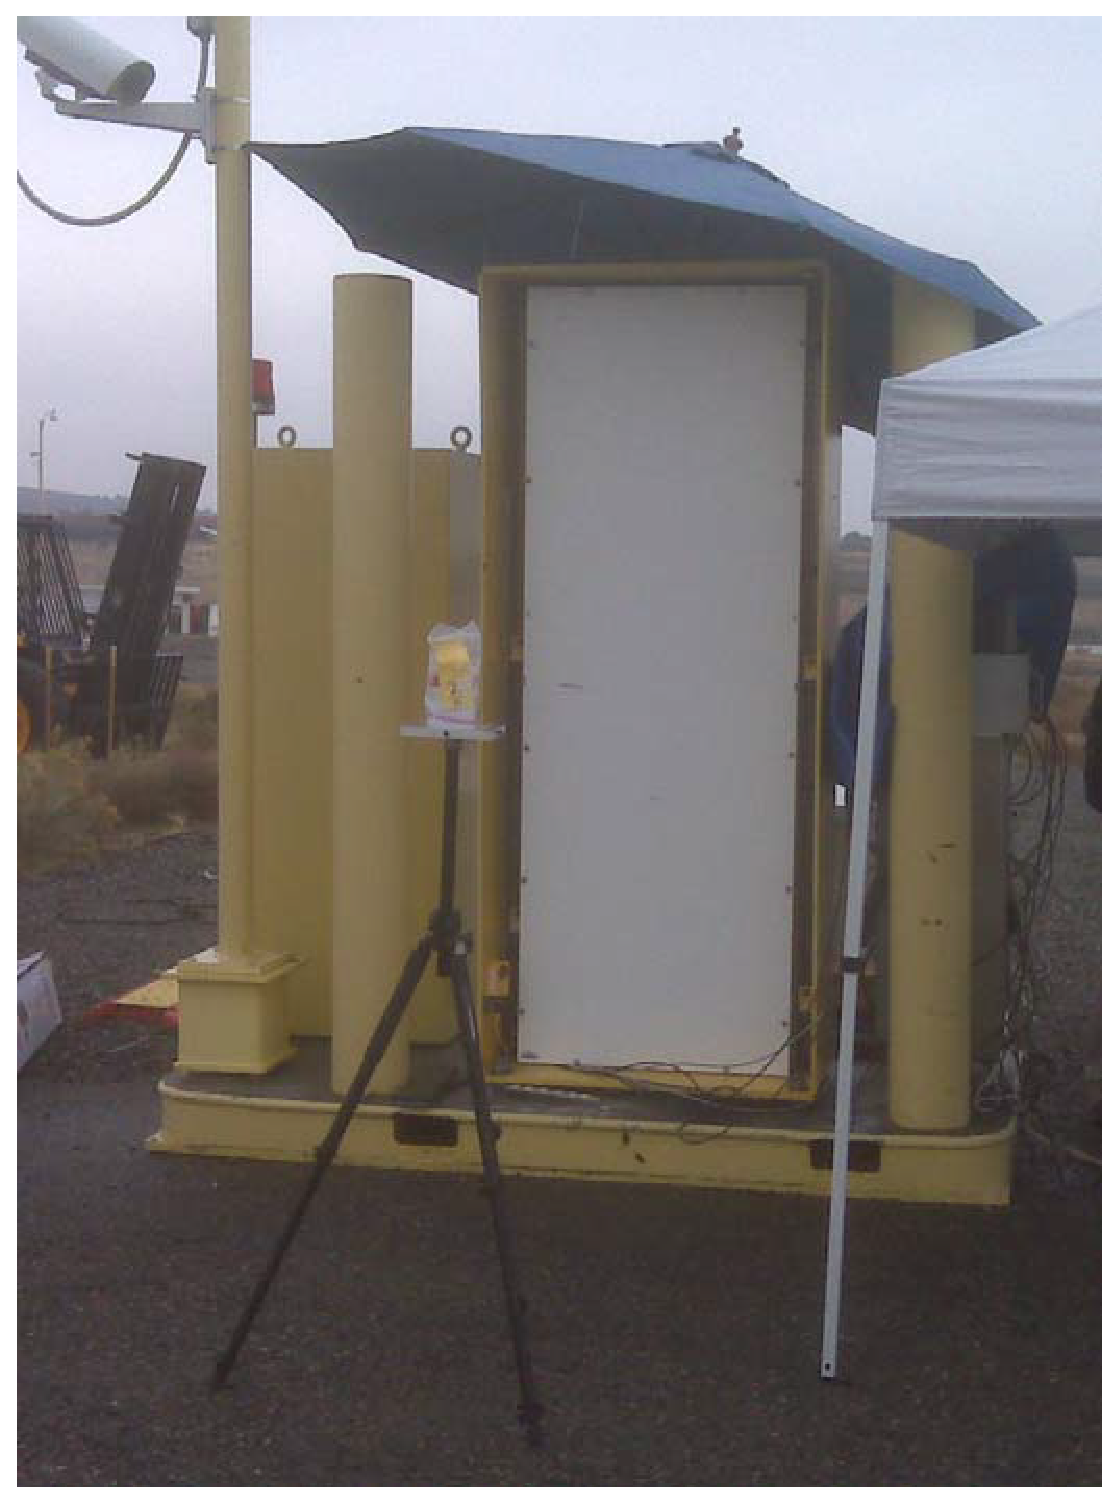
\includegraphics[height=0.25\textheight]{images/BF3Test.eps}
		\caption{PNNL test of BF${}_3$ Detector}
		\label{fig:BF3PNNLTest}
	\end{figure}
\end{column}
\end{columns}
\end{frame}

%%%%%%%%%%%%%%%%%%%%%%%%%%%%%%%%%%%%%%%%%%%%%%%%%%%%%%%%%%%%%%%%%%%%%%%%%%%%%%%
\begin{frame}{Replacement Technologies (Lithium)}
\begin{columns}[onlytextwidth]
\begin{column}{0.45\textwidth}
\begin{itemize}
	\small
	\item LiF:ZnS coated Paddles (IAT) \cite{kouzes_lithium_2010}
	\begin{itemize}
		\item Did not fulfill the neutron count rate
		\item Adequate gamma ray rejection
		\item Passed the GARRn
	\end{itemize}
	\small
	\item NucSafe Glass Fibers\cite{kouzes_alternative_2010}
	\begin{itemize}
		\item Tested with a scale model, 1.72 cps
		\item Three filter levels for GARRn
		\begin{itemize}
			\tiny
			\item Conservative filter passed GARRn, failed count rate
			\item Other filters failed GARRn
		\end{itemize}
	\end{itemize}
\end{itemize}
\end{column}
\begin{column}{0.45\textwidth}
	\begin{figure}
		\includegraphics[height=0.25\textheight]{images/LiFZnSPaddle.eps}
		\caption{${}^6$LiF:ZnS Paddle}
		\label{fig:LifZnSPaddle}
		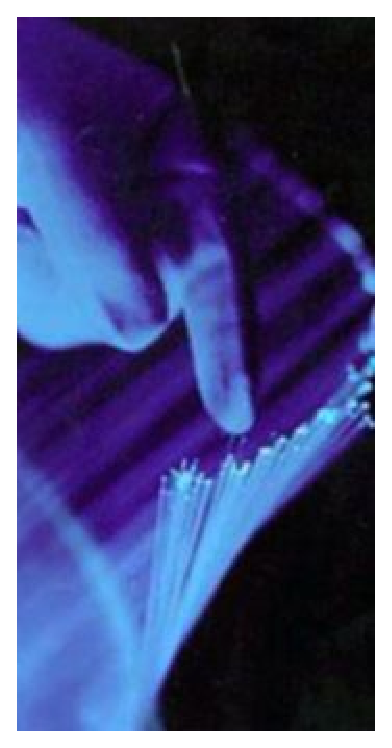
\includegraphics[height=0.25\textheight]{images/NucSafeFibers.eps}
		\caption{NucSafe Fibers}
		\label{fig:NucSafeFibers}
	\end{figure}
\end{column}
\end{columns}
\end{frame}
